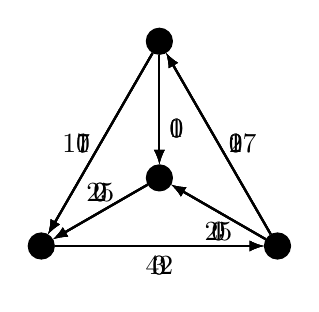
\begin{tikzpicture}[auto,scale=0.5]

	\node (c0) [circle, draw, fill=black] at (0, 0) {};
	\node (c1) [circle, draw, fill=black] at (6, 0) {};
	\node (c2) [circle, draw, fill=black] at (3, 5.2) {};
	\node (c3) [circle, draw, fill=black] at (3, 1.73) {};

	\path<1>
	(c0) edge[-latex, thick] node[below] {$42$} (c1)
	(c1) edge[-latex, thick] node[right] {$17$} (c2)
	(c2) edge[-latex, thick] node[below right] {$0$} (c3)
	(c2) edge[-latex, thick] node[left] {$17$} (c0)
	(c3) edge[-latex, thick] node[above] {$25$} (c0)
	(c1) edge[-latex, thick] node[below] {$25$} (c3);
	
	\path<2>
	(c0) edge[-latex, thick] node[below] {$0$} (c1)
	(c1) edge[-latex, thick] node[right] {$0$} (c2)
	(c2) edge[-latex, thick] node[below right] {$0$} (c3)
	(c2) edge[-latex, thick] node[left] {$0$} (c0)
	(c3) edge[-latex, thick] node[above] {$0$} (c0)
	(c1) edge[-latex, thick] node[below] {$0$} (c3);
	
	\path<3>
	(c0) edge[-latex, thick] node[below] {$3$} (c1)
	(c1) edge[-latex, thick] node[right] {$2$} (c2)
	(c2) edge[-latex, thick] node[below right] {$1$} (c3)
	(c2) edge[-latex, thick] node[left] {$1$} (c0)
	(c3) edge[-latex, thick] node[above] {$2$} (c0)
	(c1) edge[-latex, thick] node[below] {$1$} (c3);

\end{tikzpicture}
